\subsection*{Derivation of Differential Equation of Motion}
\begin{figure}[H]
	\begin{center}
		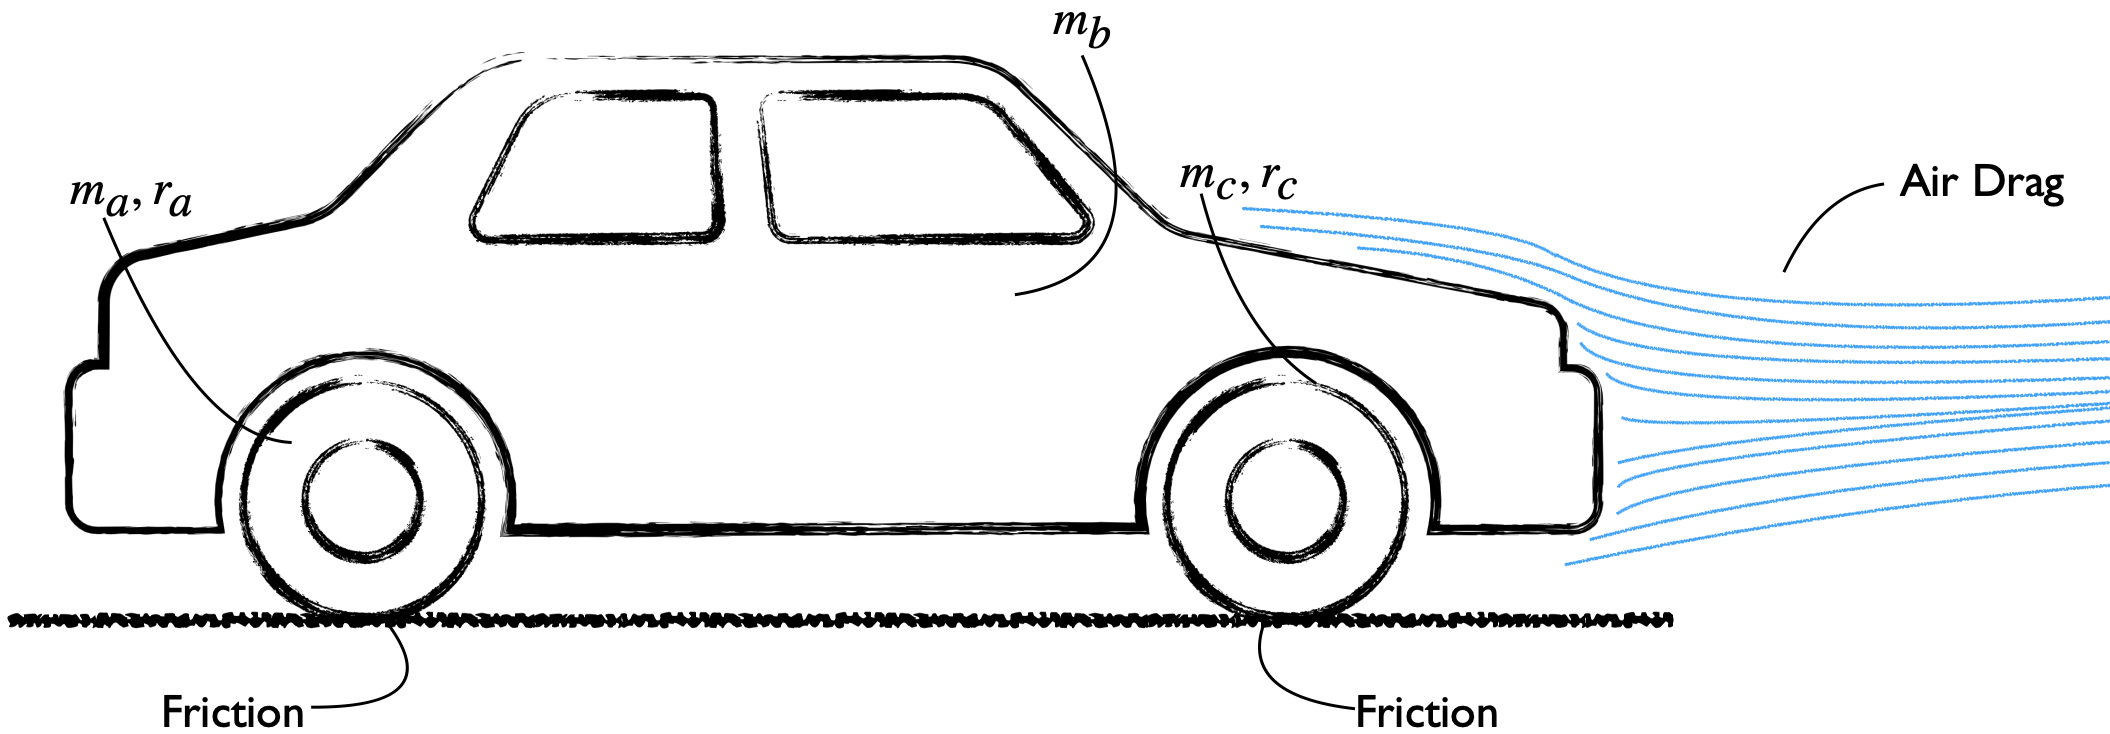
\includegraphics[width=\linewidth]{car.png}
	\end{center}
	\caption{Simplified Car Dynamics Model with Resistive Forces}
\end{figure}
We will now cut the bodies free according to d'Alembert's principle. We do so to establish the motion equation for the whole system by balancing the forces. If done correctly every force should account to the motion differential equation.
\begin{figure}[H]
	\begin{center}
		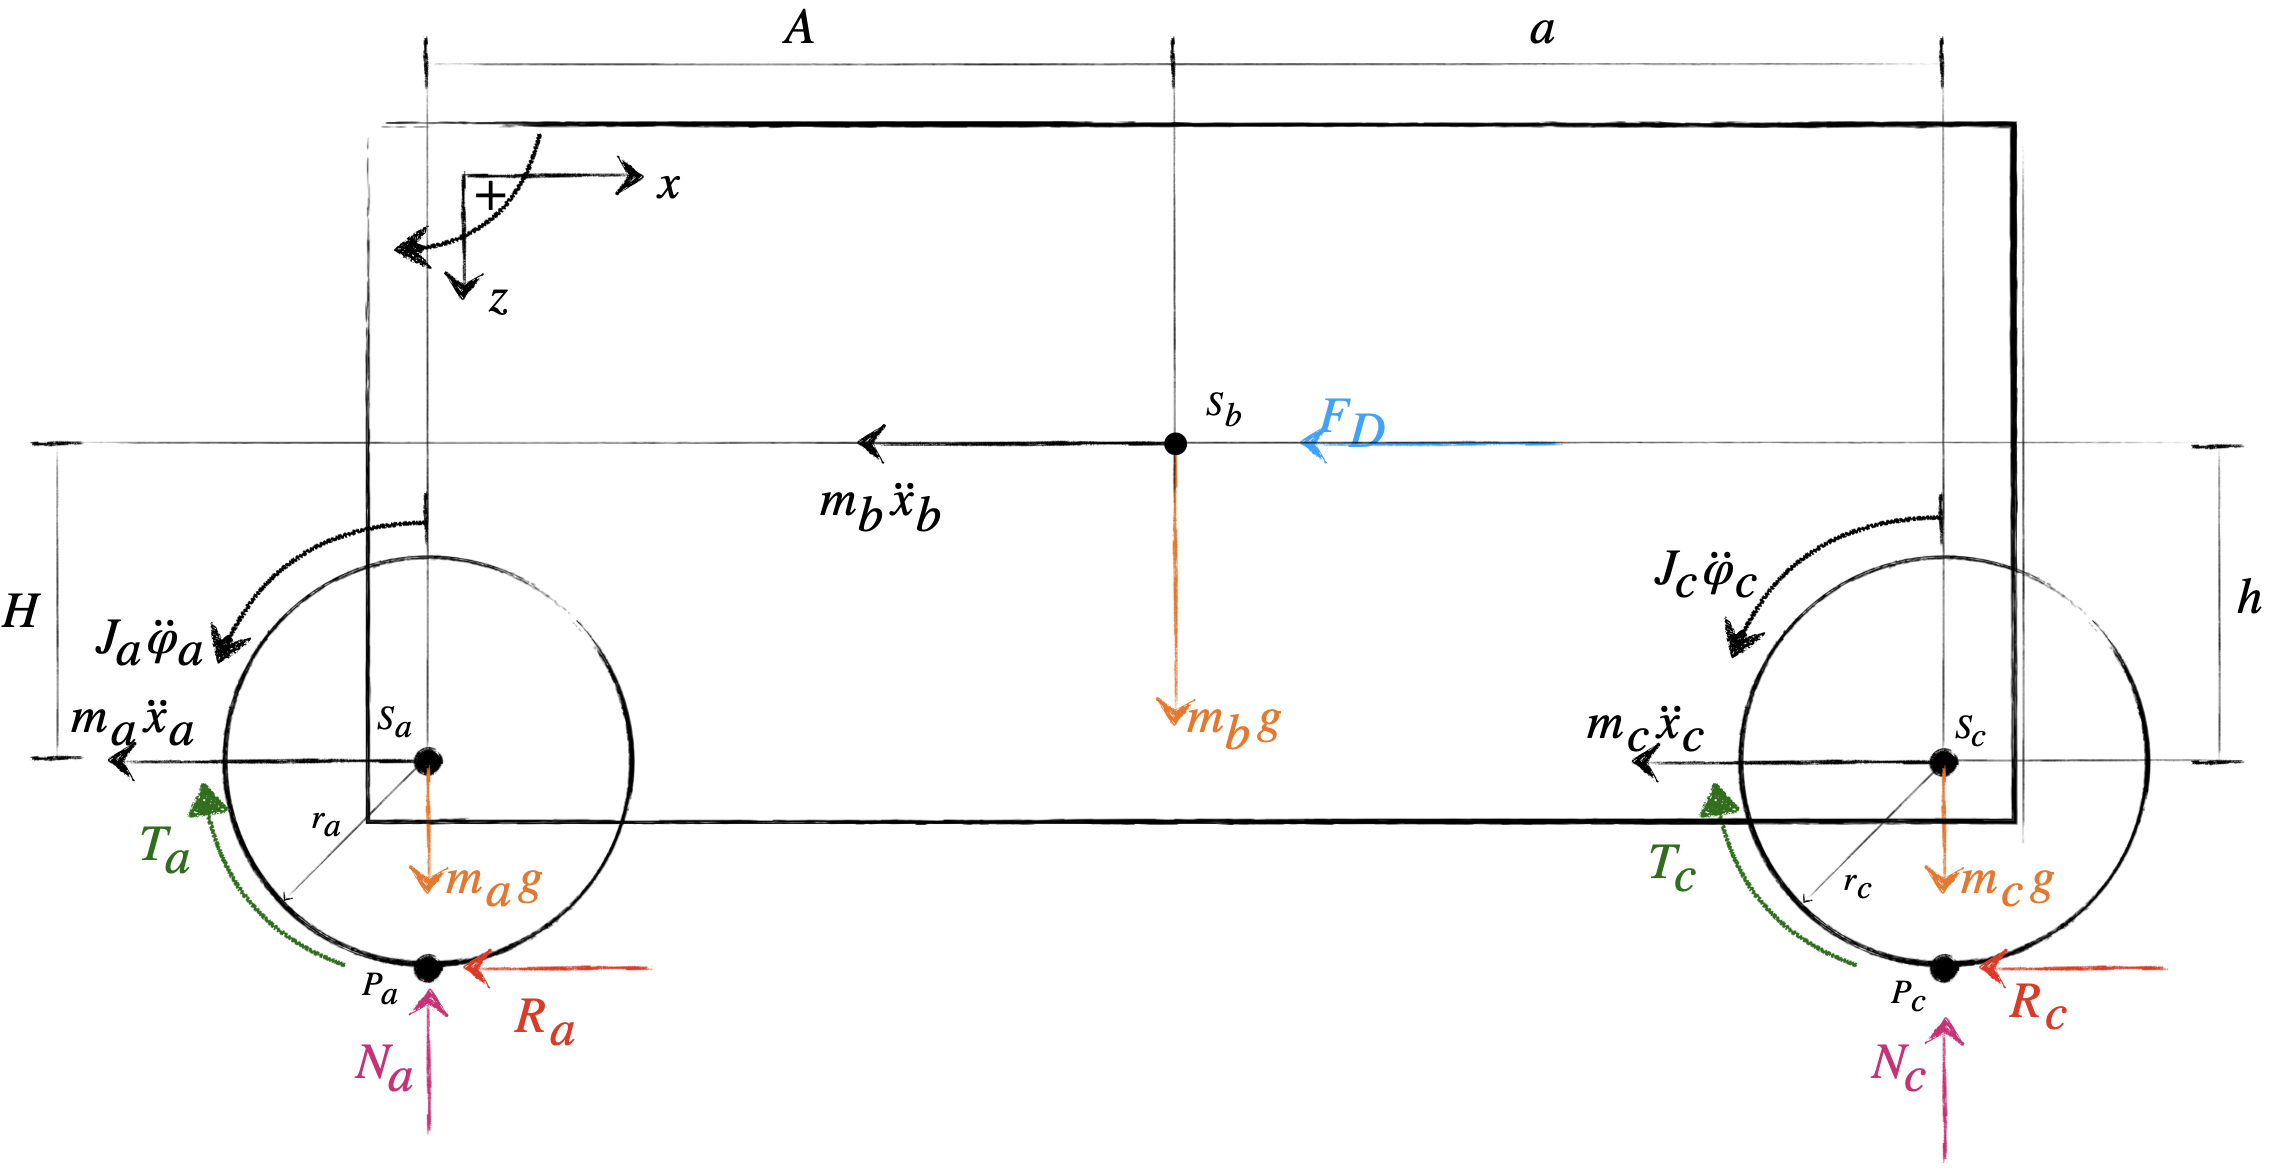
\includegraphics[width=\linewidth]{whole.png}
	\end{center}
	\caption{Forces Acting on the Vehicle (d'Alembert's Principle)}
\end{figure}
Before proceeding further, we should examine the car's kinematics. The wheels and the body are interconnected, meaning they move together as a single system. As a result, they share the same translation vector $x$ with different reference points i.e. $x=x_a=x_b=x_c$. We assume to slip-condition, hence all derivatives of $x$ (e.g., velocity and acceleration) are identical for the wheels and the body. Thus the velocity and accleration of the wheels can be simplified to: $\dot x = \dot\varphi_ar_a = \dot\varphi_cr_c$ and $\ddot x = \ddot\varphi_ar_a = \ddot\varphi_cr_c$.
\begin{multicols}{2}
	\begin{figure}[H]
		\begin{center}
			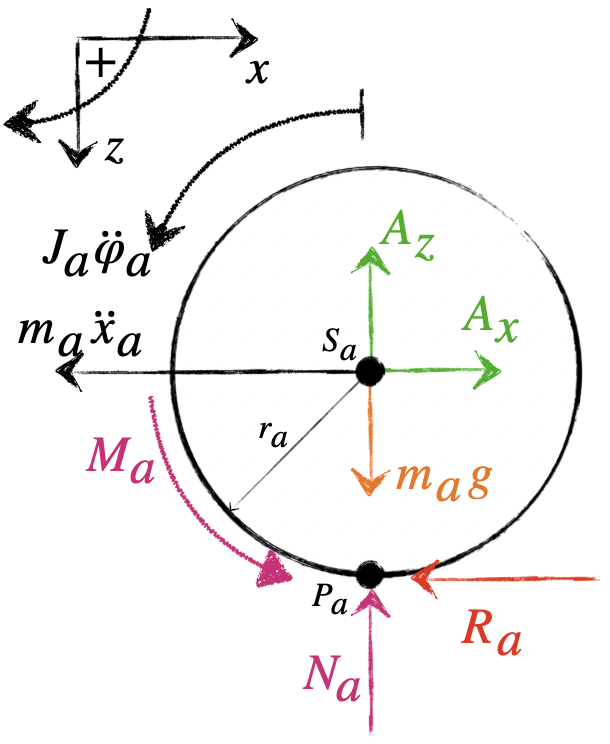
\includegraphics[width=.6\linewidth]{wheel_a.png}	
		\end{center}
		\caption{Rear Wheel $a$}
	\end{figure}
	\begin{align} \label{eq: F_xa}
     	\sum F_x:&& A_x = m_a\ddot x+R_a\\ \label{eq: F_za}
    	\sum F_z: && A_z = m_a g - N_a \\ \nonumber
	    \sum M^{\left(P_a\right)}: &&
    	J_a^{P_a}\ddot\varphi_a = \left[A_x-m_a\ddot x_a \right]r_a-T_a\\ \label{eq: M_xa}
    	&& \frac{3}{2}m_a\ddot x_a = (A_x-m_a\ddot x_a)r_a - T_a
	\end{align}
	With (\ref{eq: F_xa}) in (\ref{eq: M_xa}) follows: % equation F_x and M^{P_a}
	\begin{equation}
	    \frac{2}{3}\left(R_a - \frac{T_a}{r_a} \right) = m_a r_a\ddot \varphi_a = m_a\ddot x
    	\label{eq: m1x1}
	\end{equation}
\end{multicols}
\begin{multicols}{2}
	\begin{figure}[H]
		\begin{center}
			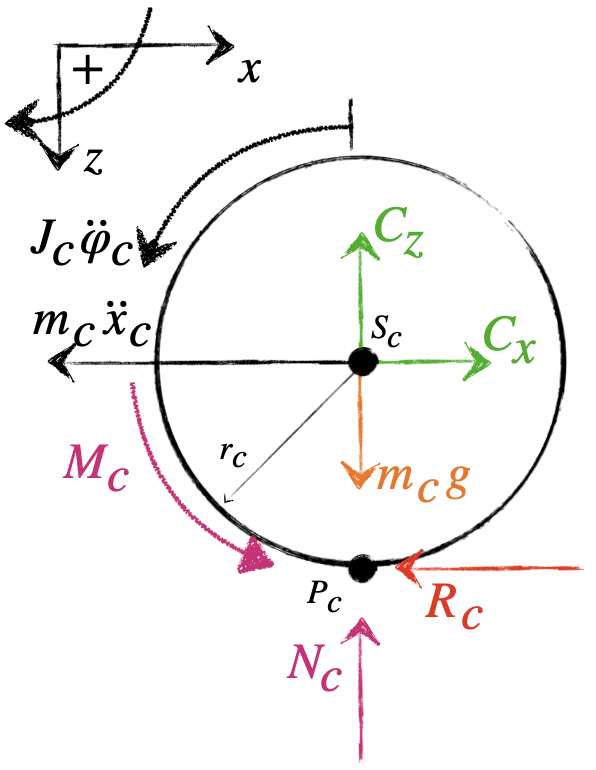
\includegraphics[width=.6\linewidth]{wheel_c.png}
		\end{center}
		\caption{Front Wheel $c$}
	\end{figure}
	\begin{align} \label{eq: F_xc}
     	\sum F_x:&& C_x = m_c\ddot x+R_c\\ \label{eq: F_zc}
    	\sum F_z: && C_z = m_c g - N_c \\ \nonumber
	    \sum M^{\left(P_c\right)}: &&
    	J_c^{P_c}\ddot\varphi_c = \left[C_x-m_c\ddot x_c \right]r_c-T_c\\ \label{eq: M_xc}
    	&& \frac{3}{2}m_c\ddot x_c = (C_x-m_c\ddot x_c)r_c - T_c
	\end{align}
	With (\ref{eq: F_xc}) in (\ref{eq: M_xc}) follows: % equation F_x and M^{P_a}
	\begin{equation}
	    \frac{2}{3}\left(R_c - \frac{T_c}{r_c} \right) = m_c r_c\ddot \varphi_c = m_c\ddot x
    	\label{eq: m2x2}
	\end{equation}
\end{multicols}

Bodywork:
\begin{multicols}{2}
	\begin{figure}[H]
		\begin{center}
			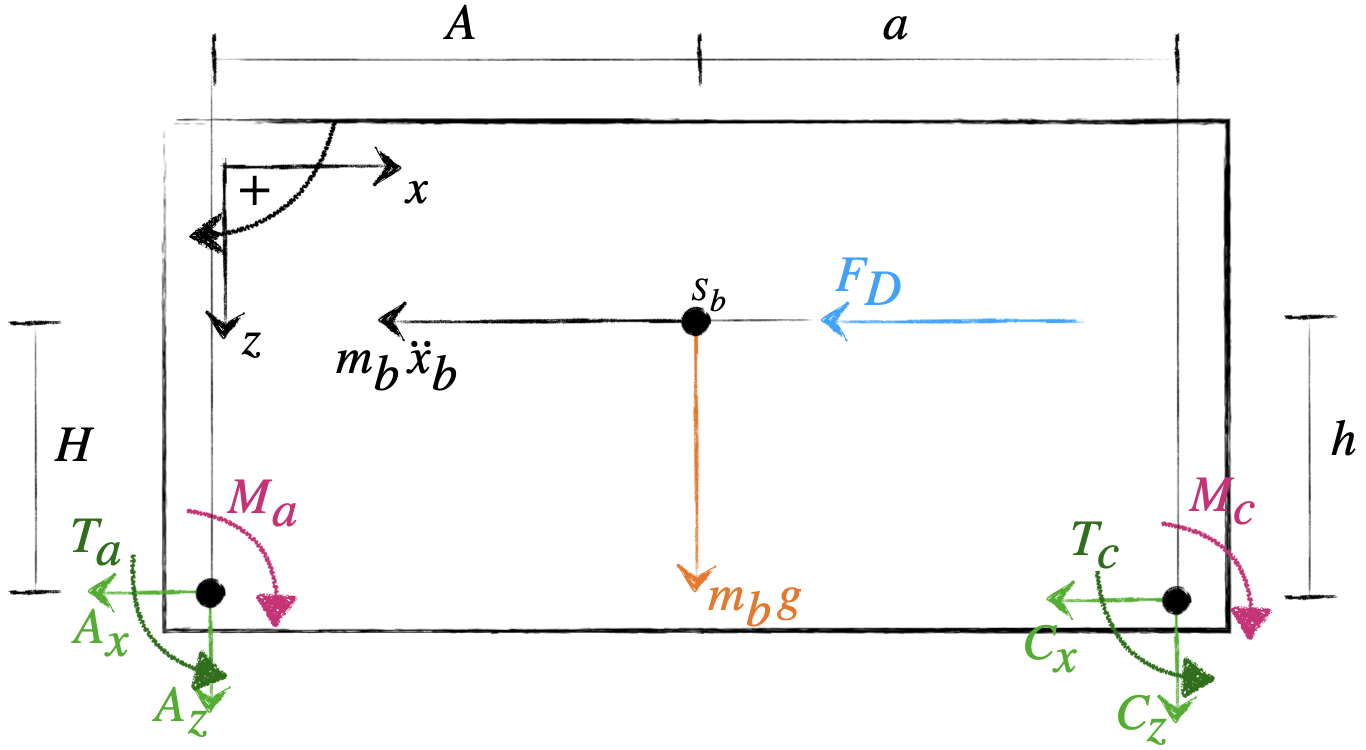
\includegraphics[width=\linewidth]{frame.png}
		\end{center}
		\caption{Bodywork}
	\end{figure}
	\begin{align} \label{eq: F_xbf}
	    \sum F_x: && m_b\ddot x = -A_x - C_x - F_D \\ \label{eq: F_zbf}
    	\sum F_z: && m_bg + A_Z +C_z = 0
	\end{align}
	(\ref{eq: F_xa}), (\ref{eq: F_xc}), (\ref{eq: F_za}) and (\ref{eq: F_zc}) into (\ref{eq: F_xbf}) and (\ref{eq: F_zbf}):
	\begin{align} \label{eq: mddx}
	    \left(m_a + m_b + m_c\right)\ddot x & = -R_a - R_c - F_D\\\label{eq: mgNaNc} 
    	(\underbrace{m_a + m_b + m_c}_{=m})g & = mg = N_a + N_c
	\end{align}
\end{multicols}
(\ref{eq: m1x1}), (\ref{eq: m2x2}) into (\ref{eq: mddx}):
\begin{align}
    m_b\ddot x &= -\frac{5}{3}\left(R_a+R_c\right) + \frac{2}{3}\left(\frac{T_a}{r_a} + \frac{T_c}{r_c}\right)- F_D
\end{align}
\begin{align}\label{eq: M_bf}
	\sum M^{(S_b)}: && C_xh + A_xH + C_za + T_a + T_c - A_za = 0
\end{align}
(\ref{eq: F_xa}), (\ref{eq: F_xc}), (\ref{eq: F_za}) and (\ref{eq: F_zc}) into (\ref{eq: M_bf}):
\begin{equation} \label{eq: M_bf2}
	h(m_c\ddot x + R_c) + H(m_a\ddot x+R_a) + (m_cg-N_c)a - (m_ag-N_a)a + T_a+T_c = 0
\end{equation}
We will assume that the distance from the center of mass is equal and the  difference in heights are negligible, hence $A=a$ and $H\approx h$. The eq. (\ref{eq: M_bf2}) takes the form:
\begin{equation} \label{eq: M_bf3}
	N_c - N_a -\frac{h}{a}(R_a+R_c) = (m_a - m_c)g + \frac{T_a+T_c}{a} + \frac{h}{a}(m_c+m_a)\ddot x
\end{equation}

The tractive force $F_T$ is the force that propels a vehicle forward by generating motion at the tire–ground interface. It is related to the torque at the wheel $T$ through:
\begin{equation*}
	T = F_T\cdot r,
\end{equation*}
where $r$ is the effective rolling radius of the tire. This relation assumes an idealized system without drivetrain losses; efficiency factors and gear ratios are incorporated in later sections.
\begin{equation} \label{eq: M_bf3}
	N_c - N_a -\frac{h}{a}(R_a+R_c) = (m_a - m_c)g + \frac{F_Tr_a+F_Tr_c}{a} + \frac{h}{a}(m_c+m_a)\ddot x
\end{equation}
The rolling resistance force $R$ arises from the interaction between the tire and the ground, primarily due to the deformation of both the tire and the surface. When the engine applies torque to the wheels, resulting in a tractive force at the contact patch, rolling resistance is present. It is commonly modeled as
\begin{equation*}
	R = c_R N,
\end{equation*}
where $c_R$ is the rolling resistance coefficient and $N$ the normal force. For our analysis, we adopt the value for the coefficient of $0.12$, as the findings of \parencite{wargula2019determination} indicated this value as the most recurrent for motor vehicles with pneumatic tires on asphalt/concrete surfaces.
\begin{equation*}
	c_R = 0.12
\end{equation*}
\\
The drag force air-resistance is given by: 
\begin{equation*}
	F_D(v) = \frac{1}{2}\rho_a c_D A_F v^2,
\end{equation*}
where $\rho_a$ is the specific air density, $c_D$ is the drag coefficient, $A_F$ is the effective frontal area $A_F$ and $v$ is the relative velocity. The Drag Coefficient $c_D$ depends on the shape of and aerodynamic properties of the vehicle. A typical value for the frontal area $A_F$ is approximately $2\text{m}^2$.
	
The air density $\rho_A$ depends on the ambient conditions and can be approximated by 
\begin{equation*}
	\rho_a = \frac{0.0348p}{T},
\end{equation*}
where $p$ is the atmosphere pressure and $T$ - the temperature. For standard conditions ($p= 1$ bar and $T= 15\degree C=288.15K$), this yields an air density of $1.225kg/m^3$ \parencite[p. 135]{mashadi2012vehicle}. 
	
Since velocity is the time derivative of position, i.e. $v=\dot x$, the drag force can also be expressed as:
\begin{equation*}
	F_D = \frac{1}{2}\rho_a c_D A_F \dot x^2.
\end{equation*}
\\
Vehicles can be equipped with either all-wheel drive (AWD) or two-wheel drive (TWD) systems, the latter being subdivided into front-wheel drive (FWD) and rear-wheel drive (RWD). Our model assumes an AWD configuration. Why is this important? Because the number and position of driven wheels directly influence the distribution of tractive force and frictional load across the tires.
	
In TWD systems, only two wheels receive torque. In FWD vehicles, the front tires are responsible for both steering and propulsion, which can lead to understeering behavior under heavy acceleration. In contrast, RWD vehicles transmit torque through the rear wheels, often offering better weight distribution during acceleration but less traction on slippery surfaces.
	
From a modeling perspective, non-driven wheels do not contribute to propulsion and thus experience no tractive friction. They primarily support the vehicle's weight and may generate rolling resistance. In AWD systems, torque is distributed across all wheels, which changes how forces—particularly tractive and rolling resistances—are shared among the tires. This impacts the overall force balance and must be accounted for in the dynamics.
	
We proceed to the distinction between them using the eq. (\ref{eq: mgNaNc}) and (\ref{eq: M_bf3}).
\begin{enumerate}
    \item RWD: $R_c, W_c, M_c = 0$ and $R_a=c_RN_a$
        \begin{align} \nonumber
            N_c & = mg - N_a\\ \label{eq: FWD_Na}
            N_a & = \frac{(2m_a + m_b)g - \frac{F_Tr_a}{a} - (m_c+m_a)\frac{h}{a}\ddot x}{2+\frac{h}{a}c_R}
        \end{align}
    \item FWD: $R_a, m_a, W_a = 0$ and $R_c=c_RN_c$
        \begin{align} \nonumber
            N_a & = mg - N_c\\ \label{eq: FWD_Nc}
            N_c & = \frac{(2m_a + m_b)g + \frac{F_Tr_c}{a} + (m_c+m_a)\frac{h}{a}\ddot x}{2-\frac{h}{a}c_R}
		\end{align}
        
    \item AWD: $R_a=c_RN_a$ and $R_c=c_RN_c$
        \begin{equation}
            N_a + N_c  = mg \label{eq: AWD_Nac}
        \end{equation}
\end{enumerate}
The differential equation of motion for each Drive type takes up the following forms:
\\
Rear-Wheel Drive:
\begin{equation}
    \left(m_b - \frac{5}{3}\cdot\frac{m_c+m_a}{2a + hc_R}c_Rh\right)\ddot x  = -\frac{5}{3}\cdot\frac{2m_a + m_b}{2 + \frac{h}{a}c_R}c_Rg + \left(\frac{2}{3} + \frac{5}{3}\cdot\frac{c_Rr_a}{2a+hc_R}\right)F_T - \frac{1}{2}\rho_a c_D A_F \dot x^2
\end{equation}
Front-Wheel Drive:
\begin{equation}
	\left(m_b + \frac{5}{3}\cdot\frac{m_c+m_a}{2a - hc_R}c_Rh\right)\ddot x  = -\frac{5}{3}\cdot\frac{2m_c + m_b}{2 - \frac{h}{a}c_R}c_Rg + \left(\frac{2}{3} - \frac{5}{3}\cdot\frac{c_Rr_c}{2a-hc_R}\right)F_T - \frac{1}{2}\rho_a c_D A_F \dot x^2
\end{equation}
All-Wheel Drive:
\begin{equation}
    m_b\ddot x = -\frac{5}{3}c_Rmg + \frac{4}{3}F_T - \frac{1}{2}\rho_a c_D A_F \dot x^2
\end{equation}

\begin{align*}
	F_{T,RWD} & = \frac{\frac{5}{3}\cdot\frac{2m_a + m_b}{2 + \frac{h}{a}c_R}c_Rg + \frac{1}{2}\rho_a c_D A_F \dot x^2 + \left(m_b - \frac{5}{3}\cdot\frac{m_c+m_a}{2a + hc_R}c_Rh\right)\ddot x}{\frac{2}{3} + \frac{5}{3}\cdot\frac{c_Rr_a}{2a+hc_R}}\\
	F_{T,FWD} & = \frac{ \frac{5}{3}\cdot\frac{2m_c + m_b}{2 - \frac{h}{a}c_R}c_Rg + \frac{1}{2}\rho_a c_D A_F \dot x^2 + \left(m_b + \frac{5}{3}\cdot\frac{m_c+m_a}{2a - hc_R}c_Rh\right)\ddot x}{\frac{2}{3} - \frac{5}{3}\cdot\frac{c_Rr_c}{2a-hc_R}}\\
	F_{T,AWD} & = \frac{3}{4}\left(\frac{5}{3}c_Rmg  + \frac{1}{2}\rho_a c_D A_F \dot x^2 + m_b\ddot x\right)
\end{align*}

Now we express the Forces as in the form of $F(t) = A + B\dot x + C\dot x^2 + D\ddot x$:

\begin{align*}
	F_{T,RWD} & = \frac{5\cdot\frac{2m_a + m_b}{2 + \frac{h}{a}c_R}c_Rg}{2 + \frac{5c_Rr_a}{2a+hc_R}}  + \frac{3\rho_a c_D A_F}{4 + \frac{10c_Rr_a}{2a+hc_R}}\dot x^2 + \frac{3m_b - 5\cdot\frac{m_c+m_a}{2a + hc_R}c_Rh}{{2 + \frac{5c_Rr_a}{2a+hc_R}}}\ddot x \\
	F_{T,FWD} & = \frac{ 5\cdot\frac{2m_c + m_b}{2 - \frac{h}{a}c_R}c_Rg}{2 - \frac{5c_Rr_c}{2a-hc_R}}  + \frac{3\rho_a c_D A_F}{4 - \frac{10c_Rr_c}{2a-hc_R}}\dot x^2 + \frac{3m_b + 5\cdot\frac{m_c+m_a}{2a - hc_R}c_Rh}{2 - 5\cdot\frac{c_Rr_c}{2a-hc_R}}\ddot x \\
	F_{T,AWD} & = \frac{5}{4}c_Rmg  + \frac{3}{8}\rho_a c_D A_F \dot x^2 + \frac{3}{4}m_b\ddot x
\end{align*}

\subsection*{Algorithms}
	\begin{algorithm}[H]
		\caption{Engine Mode Determination for Hybrid Vehicles}
		\label{alg: hyb_cond}
		\begin{algorithmic}
			\Require Acceleration array $a$, velocity array $v$
			\Ensure Condition array $cond$, where $1$: electric engine, $-1$: combustion engine
			\For{$i = 0$ to $n-1$}
			    \If{$v[i] \cdot 3.6 < 16$}
			        \State $cond[i] \gets 1$
			    \ElsIf{$a[i] < 2$}
			        \State $cond[i] \gets 1$
			    \ElsIf{$a[i] = 0$ \textbf{and} $v[i] \cdot 3.6 \leq 50$}
			        \State $cond[i] \gets 1$
			    \ElsIf{$a[i] \cdot v[i] < 0$}
			        \State $cond[i] \gets 1$
			    \Else
			        \State $cond[i] \gets -1$
			    \EndIf
			\EndFor
			\State \Return $cond$
		\end{algorithmic}
	\end{algorithm}
	
	\begin{algorithm}
		\caption{Hybrid Vehicle Energy Calculation}
		\label{alg: hyb_energy}
		\begin{algorithmic}
			\Require Time vector $t$, velocity $v$, acceleration $a$, power demand $P$, total power $P_T$
			\Require Battery capacity $E_b$, minimum State of Charge $SoC$, efficiencies $\eta_{\text{pt}}, \eta_{\text{gas}}, \eta_{\text{reg}}$
			\Ensure Total energy $W$, combustion engine energy $W_{\text{comb}}$, battery energy $W_{\text{bat}}$
			\State Compute $\Delta t_i \gets t_{i+1} - t_i$, and set $\Delta t_{n} \gets \Delta t_{n-1}$
			\State Initialize $bat \gets 0$, $ice \gets 0$
			\State Initialize arrays $W\_bat \gets 0$, $W\_ice \gets 0$
			\State Compute $cond \gets \text{cond\_hyb}(a, v)$

			\For{$i = 0$ to $n-1$}
			    \State $p \gets P[i]$, $pt \gets P_T[i]$
			    \If{$a[i] \cdot v[i] \geq 0$} \Comment{Motoring phase}
			        \If{$cond[i] = 1$ \textbf{and} $bat \leq (1 - S) \cdot E_b$}
		    	        \State $bat \gets bat + \dfrac{p}{\eta_{\text{pt}}} \cdot \dfrac{\Delta t_i}{3.6 \cdot 10^6}$
			        \Else
			            \State $ice \gets ice + \dfrac{p}{\eta_{\text{gas}}} \cdot \dfrac{\Delta t_i}{3.6 \cdot 10^6}$
			        \EndIf
			    \Else \Comment{Braking phase}
			        \State $bat \gets bat - pt \cdot \eta_{\text{reg}} \cdot \dfrac{\Delta t_i}{3.6 \cdot 10^6}$
			    \EndIf
			    \State $W\_bat[i] \gets bat$
			    \State $W\_ice[i] \gets ice$
			\EndFor
			\State $W \gets W\_bat + W\_ice$
			\State \Return $W$, $W\_ice$, $W\_bat$
		\end{algorithmic}
	\end{algorithm}
	
\subsection*{Fuel Consumption Data Frame}
	\begin{figure}[H]
		\begin{center}
			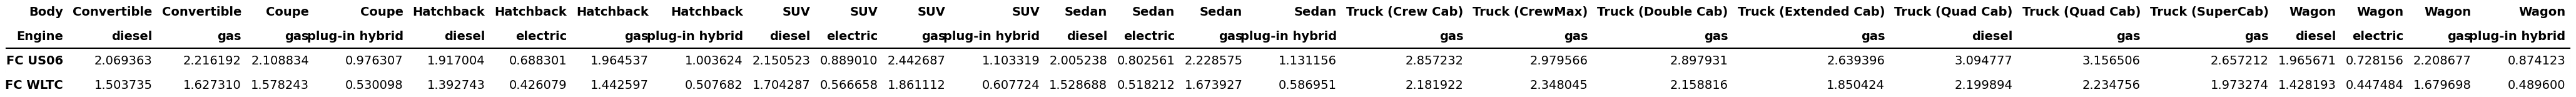
\includegraphics[width=\linewidth]{FC.png}
		\end{center}
	\end{figure}